\section{Architecture of SipCon64}
\label{sec:architecture}

\subsection{The Proposed Construction}

We introduce \emph{SipCon64}, a new encryption design. It keeps Ascon-AEAD128's outer sponge structure intact but completely replaces its inner mixing engine. We remove Ascon's S-box and linear layers entirely, swapping them out for SipHash's SIPROUND engine. However, we keep Ascon's method for adding round constants. Everything else remains exactly the same: how data enters (rate and capacity), the padding rules, the separation flags, where the key is added, and the starting setup.

Ascon's inner math is great for physical chips but forces software to use clunky workarounds. SIPROUND uses basic math that software runs instantly, but it forces physical chips to wait on slow addition steps. By swapping the engine while keeping the outer shell the same, we can isolate the exact cost of the engine on different devices. We report these measurements in Section~\ref{sec:results}.

\subsection{Components}

\subsubsection{State}
Following Ascon's design \cite{caesar}, the internal memory (the state) is written as:
\begin{equation}
S = S_r \,\|\, S_c = x_0 \,\|\, x_1 \,\|\, x_2 \,\|\, x_3,
\label{eq:state}
\end{equation}
which is four 64-bit words totaling 256 bits. We use $\lfloor X\rfloor_{\ell}$ to mean the last bits of $X$, and $\lceil X\rceil_{\ell}$ for the first bits. We treat the state as a sequence of bytes starting at the lowest byte of $x_0$.

\subsubsection{Rate and capacity}
The state is split into an outer part ($S_r = x_0$) with $r=64$ bits, and an inner part ($S_c = x_1\Vert{}x_2\Vert{}x_3$) with $c=192$ bits. Because SIPROUND only processes four words, the total memory shrinks from Ascon's 320 bits down to 256. We have to take those missing 64 bits from somewhere. We decided to cut the rate (the data input size) to 64 bits so we could keep the capacity at 192 bits. Keeping a large capacity maintains Ascon-AEAD128's security strength. The trade-off is that each step processes less data.

\subsubsection{Key, nonce and tag}
Just like Ascon-AEAD128, the key, nonce (a single-use number), and tag are all 128 bits long. We write them as $K = K_0\Vert{}K_1$ and $N = N_0\Vert{}N_1$.

\subsubsection{Initial value}
The starting value (IV) uses the exact same layout as Ascon-AEAD128. We simply add the letter 'S' (\texttt{0x53}) at the top to indicate that it uses SipHash:
\begin{equation}
\mathit{IV} = \texttt{0x00530800806A0001}.
\label{eq:iv}
\end{equation}
Because the IV includes the specific round counts, a SipCon64 setup will never accidentally overlap or collide with a standard Ascon-AEAD128 setup.

\subsection{The Round Function and the Permutations}

\begin{figure*}[!t]
\centering
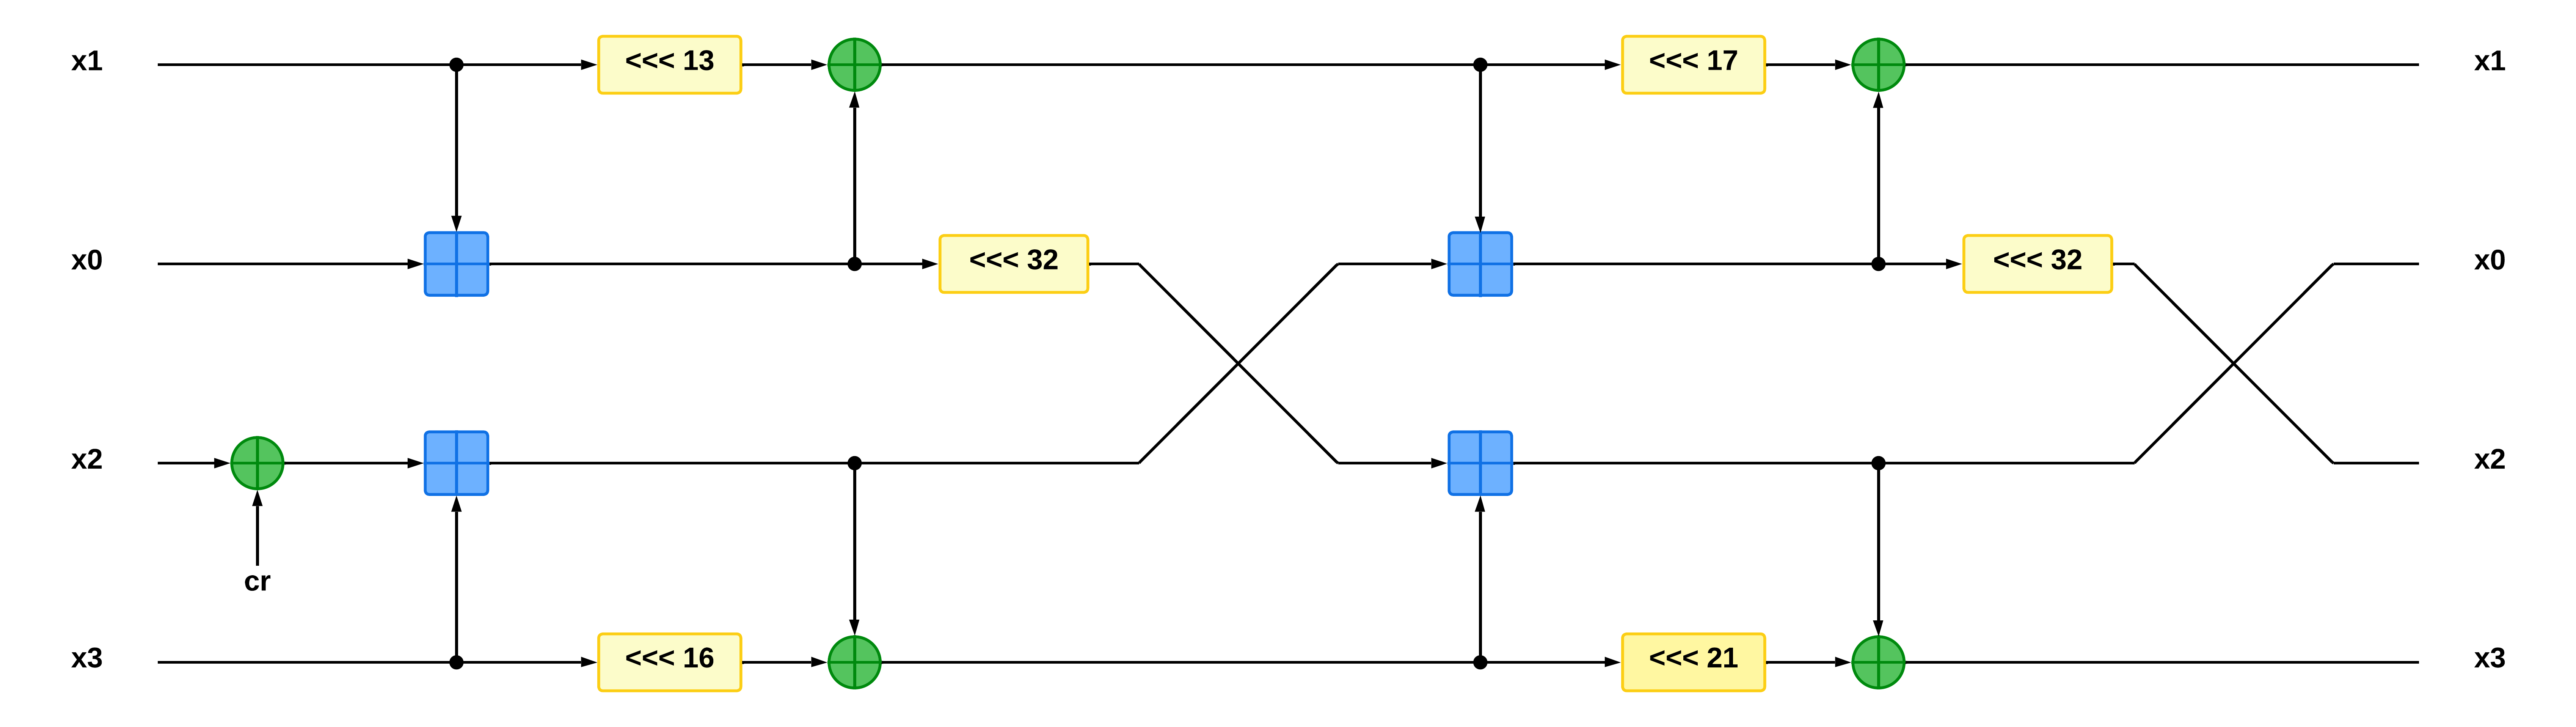
\includegraphics[width=\textwidth]{images/Round-Function}
\caption{One SipCon64 round, $p = \mathrm{SIPROUND}\circ p_C$. The round constant $c_r$ enters the capacity word $x_2$ on the left. Blue squares are additions modulo $2^{64}$, green circles are exclusive-ors, and yellow boxes are cyclic left rotations. The two additions in each half happen at the same time. The crossing in the middle happens because $x_0$ and $x_2$ switch roles in \eqref{eq:sipround}, which is swapped back on the right so the words exit in their original places.}
\label{fig:round}
\end{figure*}

\subsubsection{Symbols used in the figures}
Both diagrams use the same symbols. A plus in a square, $\boxplus$, is addition
modulo $2^{64}$; a plus in a circle, $\oplus$, is exclusive-or. A rounded box
is a cyclic left rotation by the number of positions printed inside it. A
filled dot on a wire is a fan-out, and a crossing of two wires is a relabelling
only. In Fig.~\ref{fig:mode}, a tall grey bar is a permutation call labelled
with its round count, and a slash across a wire gives that bus width in bits.

One mixing round combines two steps:
\begin{equation}
p = \mathrm{SIPROUND}\circ p_{C},
\label{eq:round}
\end{equation}
which is mapped out in Fig.~\ref{fig:round}.

\subsubsection{Constant addition}
First, $p_C$ adds a round constant to the capacity word $x_2$, just like standard Ascon \cite{caesar}:
\begin{equation}
x_2 \leftarrow x_2 \oplus c_r .
\label{eq:pc}
\end{equation}
SipCon64 uses Ascon's original twelve constants. If a phase uses fewer rounds, it takes constants from the end of the list. A 10-round mix starts at \texttt{0xd2}, and a 6-round mix starts at \texttt{0x96} (Table~\ref{tab:rc}).

\subsubsection{SIPROUND}
Next, we apply SIPROUND \cite{siphash} to the four words. We write it in two columns to show which math steps happen at the same time:
\begin{equation}
\begin{array}{ll}
x_0 \mathrel{+}= x_1 & x_2 \mathrel{+}= x_3\\
x_1 \mathrel{\lll}= 13 \qquad & x_3 \mathrel{\lll}= 16\\
x_1 \mathrel{\oplus}= x_0 & x_3 \mathrel{\oplus}= x_2\\
x_0 \mathrel{\lll}= 32 & \\[2pt]
x_2 \mathrel{+}= x_1 & x_0 \mathrel{+}= x_3\\
x_1 \mathrel{\lll}= 17 & x_3 \mathrel{\lll}= 21\\
x_1 \mathrel{\oplus}= x_2 & x_3 \mathrel{\oplus}= x_0\\
x_2 \mathrel{\lll}= 32 &
\end{array}
\label{eq:sipround}
\end{equation}
The left and right columns do not depend on each other, meaning a processor can run them simultaneously. Between the top and bottom halves, $x_0$ and $x_2$ switch partners. You can see this crossover in the middle of Fig.~\ref{fig:round}.

This layout is very important for hardware. Even though the round uses four addition steps, they do not happen one after another. The two top additions process at the same time, and the two bottom additions process at the same time. Therefore, the chip only suffers the delay of \emph{two} stacked additions per round, not four.

\subsubsection{The two permutations}
We use two different mixing strengths. We use 10 rounds ($p^{10}$) at the very beginning and end to maximize security where attackers have the most control. We use a faster 6-round mix ($p^{6}$) in the middle between data blocks.

\begin{table}[!t]
\centering
\caption{Round constants $c_r$, kept exactly as they are in Ascon. A shorter mix uses the constants at the end of the list, so $p^{10}$ starts at \texttt{0xd2} and $p^{6}$ starts at \texttt{0x96}.}
\label{tab:rc}
\small
\begin{tabular}{ccl@{\qquad}ccl}
\hline
$p^{10}$ & $p^{6}$ & $c_r$ & $p^{10}$ & $p^{6}$ & $c_r$\\
\hline
0 & & \texttt{0xd2} & 5 & 1 & \texttt{0x87}\\
1 & & \texttt{0xc3} & 6 & 2 & \texttt{0x78}\\
2 & & \texttt{0xb4} & 7 & 3 & \texttt{0x69}\\
3 & & \texttt{0xa5} & 8 & 4 & \texttt{0x5a}\\
4 & 0 & \texttt{0x96} & 9 & 5 & \texttt{0x4b}\\
\hline
\end{tabular}
\end{table}

\subsection{The Duplex Mode}

\begin{figure*}[!t]
\centering
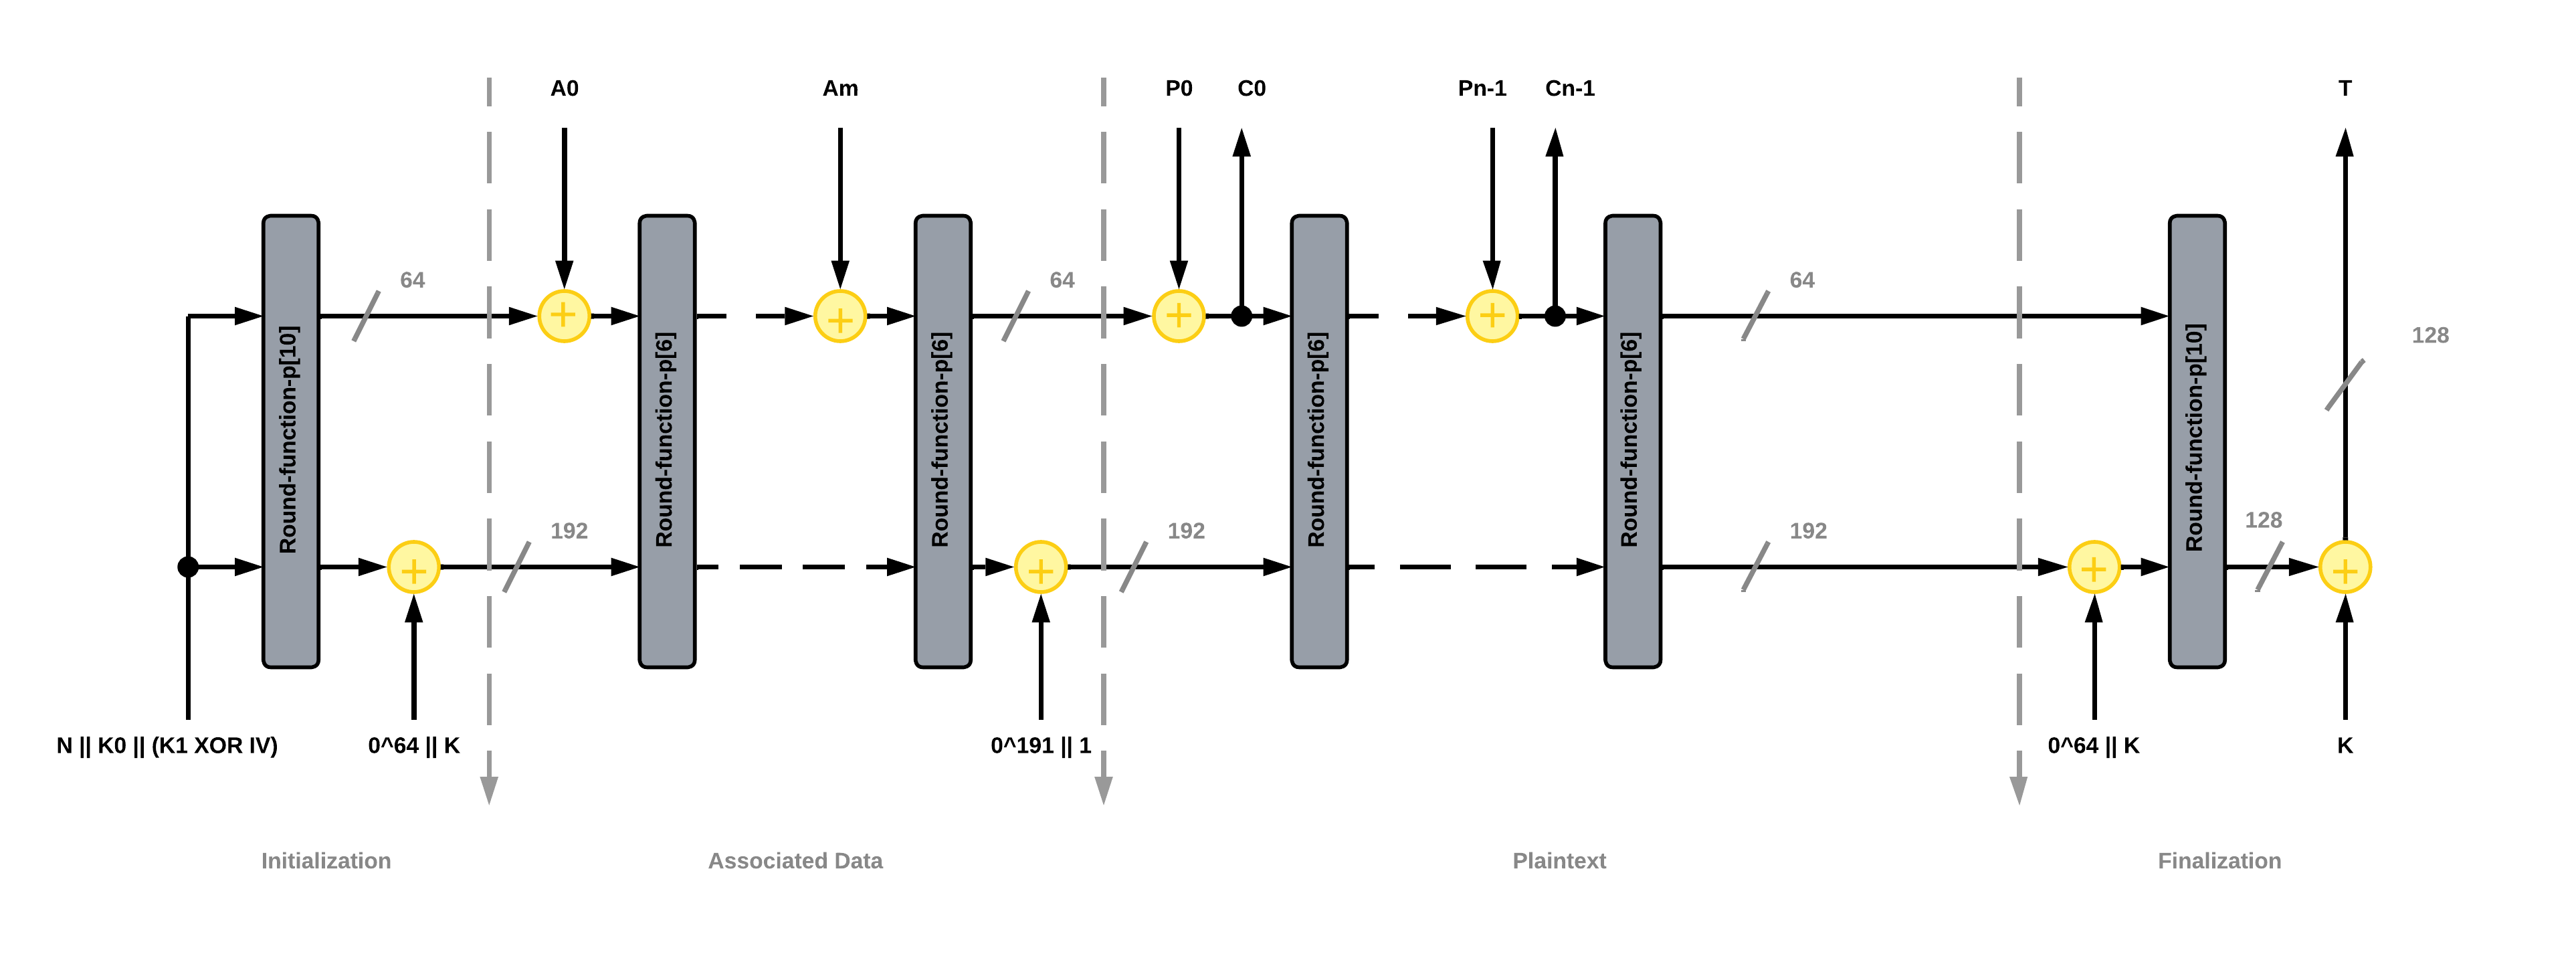
\includegraphics[width=\textwidth]{images/sipcon-mode}
\caption{SipCon64's operating mode. The top line is the 64-bit rate $x_0$, where all data enters and leaves. The bottom line is the 192-bit capacity $x_1,x_2,x_3$, which keeps the system secure by never directly touching outside data. We use $p^{10}$ at the start and end, injecting the key both times. We use $p^{6}$ between data blocks. The extra bit added before the plaintext phase is the domain separator from \eqref{eq:dsep}.}
\label{fig:mode}
\end{figure*}

Fig.~\ref{fig:mode} outlines the four main phases.

\subsubsection{Padding}
\label{sec:padding}
Two of those phases end with a block that may be only partly filled, and both
close it the same way. Padding is not a separate step in the diagram: it
happens \emph{inside} the last absorption of the associated-data phase and
again inside the last absorption of the plaintext phase, and Fig.~\ref{fig:mode}
does not draw it.

Let $\ell$ be the number of message bits in that final block, $0 \le \ell < r$.
The block is absorbed into the low $\ell$ bits of the rate, the ciphertext is
taken from those same $\ell$ bits, and a single \texttt{1} bit followed by
zeros is then exclusive-ored into the $r-\ell$ bits above them:
\begin{equation}
S_r \leftarrow S_r \oplus (0^{\ell} \,\|\, 1 \,\|\, 0^{\,r-1-\ell}).
\label{eq:pad}
\end{equation}
In the implementation this is the single byte \texttt{0x01} placed at byte
offset $\ell/8$ of $x_0$, and it is applied \emph{after} the ciphertext has
been extracted, so the padding never reaches the output. Because it touches
only bits the message did not occupy, it marks unambiguously where the data
ended and prevents two messages of different length from leaving the state in
the same condition.

Fig.~\ref{fig:mode} sets out the block structure of each phase; the padding
rule that brings every block up to $r$ bits is carried by \eqref{eq:pad} rather
than drawn. Under that rule a closing fragment of $\ell$ bits becomes the full
block $M \,\|\, 1 \,\|\, 0^{\,r-1-\ell}$, so the permutation always receives
$r$ bits whatever the message length. SipCon64 follows Ascon \cite{caesar} here
unchanged.

\subsubsection{Initialization}
We load the nonce and the key, mix the state, and then inject the key again:
\begin{align}
S &\leftarrow N_0 \,\|\, N_1 \,\|\, K_0 \,\|\, (K_1 \oplus \mathit{IV}),
\nonumber\\
S &\leftarrow p^{10}(S) \oplus (0^{128} \,\|\, K).
\label{eq:init}
\end{align}
Because SipCon64 only has four words, it does not have a spare word to hold the IV like Ascon does. Instead, it merges the IV directly into the key ($K_1$) while the nonce takes up $x_0,x_1$.

\subsubsection{Associated data}
We mix each 64-bit chunk of extra data into the rate and run 6 rounds:
\begin{equation}
S \leftarrow p^{6}\big((S_r \oplus A_i) \,\|\, S_c\big),
\qquad 1 \le i \le s,
\label{eq:ad}
\end{equation}
After all chunks are handled, we flip a single bit to separate this phase from the next:
\begin{equation}
S \leftarrow S \oplus (0^{255} \,\|\, 1).
\label{eq:dsep}
\end{equation}
Just like Ascon, we flip this bit \emph{even if there was no extra data provided}. This prevents the system from confusing an empty data phase with the start of the message. Fig.~\ref{fig:mode} shows this bit landing in the capacity section ($0^{191}\Vert{}1$), which translates to the byte \texttt{0x80} at the top of $x_3$.

\subsubsection{Plaintext}
We combine each message block with the rate to create the ciphertext output:
\begin{equation}
C_i \leftarrow S_r \oplus P_i, \qquad
S \leftarrow
\begin{cases}
p^{6}(C_i \,\|\, S_c) & 1 \le i < t\\
C_i \,\|\, S_c & i = t,
\end{cases}
\label{eq:pt}
\end{equation}
We cut the final block to the exact size of the message and do not run a mixing step afterward.

\subsubsection{Finalization}
We inject the key, mix the state a final time, and extract the tag from the last two words:
\begin{align}
S &\leftarrow p^{10}\big(S \oplus (0^{128} \,\|\, K)\big),
\nonumber\\
T &\leftarrow \lfloor S \rfloor_{128} \oplus K.
\label{eq:final}
\end{align}
Ascon injects the key into different spots before and after this final mix. SipCon64 injects the key into the exact same spot both times (the last two words, $x_2$ and $x_3$) because that is where we pull the final tag from.

\subsection{Encryption and Decryption}

Algorithms~\ref{alg:enc} and~\ref{alg:dec} detail the entire process. They only differ in one specific way: encryption mixes the message into the rate, while decryption pulls the message out and then \emph{overwrites} the rate with the ciphertext. For the final partial block, it overwrites only the needed bits while leaving the leftover padding bits untouched.

\begin{algo}{$\mathrm{SipCon64\text{-}Enc}(K, N, A, P)$}\label{alg:enc}
\areq{128-bit key $K=K_0\|K_1$, 128-bit nonce $N=N_0\|N_1$, associated data $A$, plaintext $P$}
\aens{ciphertext $C$, 128-bit tag $T$}
\aphase{Initialization phase}
\aln $x_0 \leftarrow N_0$;\ \ $x_1 \leftarrow N_1$;\ \ $x_2 \leftarrow K_0$;\ \ $x_3 \leftarrow K_1 \oplus \mathit{IV}$
\aln $S \leftarrow p^{10}(S)$
\aln $x_2 \leftarrow x_2 \oplus K_0$;\ \ $x_3 \leftarrow x_3 \oplus K_1$
\aphase{Associated data phase}
\aln \kw{if} $|A| > 0$ \kw{then}
\aln[1] $A_1 \dots A_s \leftarrow 64$-bit blocks of $A\|1\|0^{*}$
\aln[1] \kw{for} $i = 1$ \kw{to} $s$ \kw{do}
\aln[2] $x_0 \leftarrow x_0 \oplus A_i$
\aln[2] $S \leftarrow p^{6}(S)$
\aln[1] \kw{end for}
\aln \kw{end if}
\aln $x_3 \leftarrow x_3 \oplus \mathit{DSEP}$ \cmt{also if $s=0$}
\aphase{Plaintext phase}
\aln $P_1 \dots P_t \leftarrow 64$-bit blocks of $P\|1\|0^{*}$
\aln \kw{for} $i = 1$ \kw{to} $t-1$ \kw{do}
\aln[1] $C_i \leftarrow x_0 \oplus P_i$
\aln[1] $x_0 \leftarrow C_i$
\aln[1] $S \leftarrow p^{6}(S)$
\aln \kw{end for}
\aln $C_t \leftarrow x_0 \oplus P_t$;\ \ $x_0 \leftarrow C_t$ \cmt{no trailing $p^{6}$}
\aln $\tilde{C}_t \leftarrow \lfloor C_t \rfloor_{|P| \bmod r}$
\aphase{Finalization phase}
\aln $x_2 \leftarrow x_2 \oplus K_0$;\ \ $x_3 \leftarrow x_3 \oplus K_1$
\aln $S \leftarrow p^{10}(S)$
\aln $T \leftarrow (x_2 \oplus K_0) \,\|\, (x_3 \oplus K_1)$
\aunn[1] \kw{return} $C_1\|\dots\|C_{t-1}\|\tilde{C}_t$, $T$
\end{algo}

\begin{algo}{$\mathrm{SipCon64\text{-}Dec}(K, N, A, C, T)$}\label{alg:dec}
\areq{128-bit key $K=K_0\|K_1$, 128-bit nonce $N=N_0\|N_1$, associated data $A$, ciphertext $C$, tag $T$}
\aens{plaintext $P$, or $\bot$ on authentication failure}
\aphase{Initialization phase}
\aln $x_0 \leftarrow N_0$;\ \ $x_1 \leftarrow N_1$;\ \ $x_2 \leftarrow K_0$;\ \ $x_3 \leftarrow K_1 \oplus \mathit{IV}$
\aln $S \leftarrow p^{10}(S)$
\aln $x_2 \leftarrow x_2 \oplus K_0$;\ \ $x_3 \leftarrow x_3 \oplus K_1$
\aphase{Associated data phase}
\aln \kw{if} $|A| > 0$ \kw{then}
\aln[1] $A_1 \dots A_s \leftarrow 64$-bit blocks of $A\|1\|0^{*}$
\aln[1] \kw{for} $i = 1$ \kw{to} $s$ \kw{do}
\aln[2] $x_0 \leftarrow x_0 \oplus A_i$
\aln[2] $S \leftarrow p^{6}(S)$
\aln[1] \kw{end for}
\aln \kw{end if}
\aln $x_3 \leftarrow x_3 \oplus \mathit{DSEP}$ \cmt{also if $s=0$}
\aphase{Ciphertext phase}
\aln $C_1 \dots C_{t-1}\tilde{C}_t \leftarrow 64$-bit blocks of $C$, $0 \le |\tilde{C}_t| < r$
\aln \kw{for} $i = 1$ \kw{to} $t-1$ \kw{do}
\aln[1] $P_i \leftarrow x_0 \oplus C_i$
\aln[1] $x_0 \leftarrow C_i$ \cmt{rate replaced, not XORed}
\aln[1] $S \leftarrow p^{6}(S)$
\aln \kw{end for}
\aln $\ell \leftarrow |\tilde{C}_t|$
\aln $\tilde{P}_t \leftarrow \lfloor x_0 \rfloor_{\ell} \oplus \tilde{C}_t$
\aln $x_0 \leftarrow x_0 \oplus (\tilde{P}_t\|1\|0^{r-1-\ell})$ \cmt{no trailing $p^{6}$}
\aphase{Finalization phase}
\aln $x_2 \leftarrow x_2 \oplus K_0$;\ \ $x_3 \leftarrow x_3 \oplus K_1$
\aln $S \leftarrow p^{10}(S)$
\aln $T^{*} \leftarrow (x_2 \oplus K_0) \,\|\, (x_3 \oplus K_1)$
\aln \kw{if} $T^{*} \ne T$ \kw{then return} $\bot$ \cmt{constant time}
\aunn[1] \kw{return} $P_1\|\dots\|P_{t-1}\|\tilde{P}_t$
\end{algo}

\subsection{Round-per-Cycle Hardware Realization}

The hardware version runs one full round every clock cycle. It uses a single 256-bit memory register, one block of math logic, and a basic controller. Since every phase uses the exact same mixing logic, the controller simply keeps track of the current phase. A 4-bit counter picks the round constant, starting at 2 for 10 rounds and 6 for 6 rounds, counting up to 11 both times.

Data moves in and out through 64-bit ports. A simple mask handles padding instantly during the exact same step the data is mixed. Encryption and decryption share almost all the same wiring; the only difference is whether the system mixes the incoming block or overwrites the rate entirely.

Processing $n_A$ data blocks and $n_M \ge 1$ message blocks takes this many cycles:
\begin{equation}
10 + 6,n_A + 6,(n_M - 1) + 10 \ \text{cycles},
\label{eq:cycles}
\end{equation}
compared to Ascon-AEAD128's $12 + 8n_A + 8(n_M-1) + 12$ over larger blocks. Because the system runs one round per cycle, the speed is directly limited by the two addition steps stacked on top of each other (Fig.~\ref{fig:round}). We cannot remove this delay without splitting the round into multiple cycles or using less accurate math, neither of which we do here.
